\section{Results, quantity by quantity}
\label{sec:results}
\label{sec:perf}

\textbf{Purpose.} Each quantity of Table~\ref{tab:qv:qoi} in turn, with the RANS result first and
the low-order study's value beside it wherever the study produces one. Every coefficient is on the
DSO basis and every difference is formed inside one operating point; the comparison of the two
methods as a selection tool is drawn together in Section~\ref{sec:lo}.

\subsection{Trimmed drag at Condition CR}
\label{sec:cr}
\label{sec:perf:cr}
\label{sec:project:result}

\textbf{Result.} Table~\ref{tab:perf:cr} gives the low-speed result, and the headline is how
little separates the candidates. The five span \SI{1.1}{counts}, from W at $-0.868$ to M at
$+0.232$. Four of the five sit below the baseline and one above it, but every one of them is
inside a count and a half. On $L/D$ the whole field lies between 22.75 and 22.88, a spread of an
eighth of a point; W reaches $22.882$ against the baseline's $22.776$. Every candidate reaches target lift
at lower incidence than the baseline, by 0.19 to 0.50~deg: the aft camber does its intended job
at this condition.
\textbf{Ordering.} The concept ordering differs between the two points, and at low speed only
the grouping is resolvable, not the sequence within it. At Condition CR W and F are the two cheapest, separated by
$0.053$ counts, with F sitting $0.806$ counts below H; at early cruise C and M are the two
cheapest and F is the most expensive of all five. Differences of a twentieth of a count between adjacent pairs at low speed
are the size of the convergence gate itself, so the low-speed sequence is read as a group rather
than a ranking, even though the $1.1$-count spread across the whole field is twenty-two times
that gate and is real. The cruise points, where the field spans forty counts, are where
the ordering carries. Note also that C, M and F are all continuous trailing-edge camber and do
not group together at either point: the concept does not by itself decide the cost.

\begin{table}[htbp]
\centering
\footnotesize
\caption{Trimmed performance at Condition CR, $M=0.10$, target $C_L=0.428277635108$, kOmegaSST
wall resolved. DSO basis, half model, $A_\mathrm{ref}=\num{0.620462}$~m$^2$; one drag count is
$10^{-4}$. $\Delta C_D$ is against \texttt{SWB\_trim} at the same condition and the same target
lift, negative being a saving. $C_L-$tgt is in counts of $C_L$. Rank is by $\Delta C_D$, cheapest
first. Source: \texttt{data/rans\_forces.json}, rows emitted by \texttt{scripts/make\_cr\_table.py}.}
\label{tab:perf:cr}
\begin{tabular}{llrrrrrr}
\toprule
Geom. & Case & $\alpha$ (deg) & $C_D$ (ct) & $\Delta C_D$ (ct) & $C_L-$tgt (ct) & $L/D$ & Rank \\
\midrule
B & SWB\_trim & 1.7476 & 188.031 & $+0.000$ & $-0.094$ & 22.776 & -- \\
C & SWC\_trim & 1.2683 & 187.840 & $-0.191$ & $-0.005$ & 22.800 & 3 \\
M & SWM\_trim & 1.2574 & 188.263 & $+0.232$ & $+0.001$ & 22.749 & 5 \\
F & SWF\_trim & 1.4755 & 187.216 & $-0.815$ & $-0.039$ & 22.876 & 2 \\
W & SWW\_trim & 1.5205 & 187.163 & $-0.868$ & $-0.037$ & 22.882 & 1 \\
H & SWH\_trim & 1.5523 & 188.022 & $-0.009$ & $-0.039$ & 22.778 & 4 \\
\bottomrule
\end{tabular}
\end{table}

\subsection{Trimmed drag at cruise}
\label{sec:cruise}
\textbf{Purpose.} The two cruise points are early cruise at $M = 0.78$ and
$C_L = 0.529297087450$ and late cruise at $M = 0.78$ and $C_L = 0.544114800210$. The two are
separate operating points: each carries its own baseline trim, every increment is formed inside
one of them, and nothing is differenced across them or against Condition~CR. Both run
Spalart--Allmaras wall modelled where Condition~CR runs kOmegaSST wall resolved, so counts from
the two regimes are set beside one another as magnitudes only.

\subsubsection{Early cruise}
\label{sec:perf:ec}
\textbf{Result.} Table~\ref{tab:perf:ec} gives the cruise result, and it is the decision-level
one. \textbf{W is the only candidate that saves drag}, by $0.769$~counts against a baseline of
$177.839$, which raises $L/D$ from $29.764$ to $29.889$. F and H cost $1.796$ and $2.244$~counts,
$0.30$ and $0.37$ points of $L/D$. C and M cost $12.871$ and $14.554$~counts, $2.0$ and $2.3$
points of $L/D$. Every trim lands within $0.565$~ct of target $C_L$, inside the one-count
tolerance; the drag bias that residual implies is at most $0.022$~ct and is carried per case in
the data file.

\textbf{Incidence.} Each candidate again trims at lower incidence than the baseline, by $0.17$
to $0.36$~deg. The commanded camber delivers its lift at cruise as designed. The drag
consequence depends on where it puts the recompression (Section~\ref{sec:perf:mechanism}).

\begin{table}[htbp]
\centering
\footnotesize
\caption{Trimmed performance at early cruise, $M=0.78$, target $C_L=0.529297087450$,
Spalart--Allmaras wall modelled. Frame and conventions as Table~\ref{tab:perf:cr}, with the
baseline \texttt{CMPB\_trim}; rows ranked by $\Delta C_D$.
Source: \texttt{data/rans\_forces.json}, rows generated by
\texttt{scripts/make\_cruise\_tables.py}.}
\label{tab:perf:ec}
\begin{tabular}{llrrrrrr}
\toprule
Geom. & Case & $\alpha$ (deg) & $C_D$ (ct) & $\Delta C_D$ (ct) & $C_L-$tgt (ct) & $L/D$ & Rank \\
\midrule
\inputrows{sections/gen/tab_perf_ec_rows.tex}
\bottomrule
\end{tabular}
\end{table}

\subsubsection{Late cruise}
\label{sec:perf:lc}
\label{sec:perf:late}

\textbf{Result.} Table~\ref{tab:perf:lc} gives the late-cruise result, and it reproduces the
early-cruise picture. W again saves drag, by $0.781$~counts against a baseline of
$187.959$; F and H cost $1.348$ and $1.927$; C and M cost $12.214$ and $13.728$. Every trim lands
within $0.895$~ct of target $C_L$, the widest being \texttt{LCW\_trim}, and incidence again falls
below the baseline's, by $0.16$ to $0.35$~deg.
\begin{table}[htbp]
\centering
\footnotesize
\caption{Trimmed performance at late cruise, $M=0.78$, target $C_L=0.544114800210$,
Spalart--Allmaras wall modelled. Frame and conventions as Table~\ref{tab:perf:ec}, with the
baseline \texttt{LCB\_trim}. Same turbulence model and wall
treatment as early cruise, so these counts are directly comparable with
Table~\ref{tab:perf:ec}. Source as Table~\ref{tab:perf:ec}.}
\label{tab:perf:lc}
\begin{tabular}{llrrrrrr}
\toprule
Geom. & Case & $\alpha$ (deg) & $C_D$ (ct) & $\Delta C_D$ (ct) & $C_L-$tgt (ct) & $L/D$ & Rank \\
\midrule
\inputrows{sections/gen/tab_perf_lc_rows.tex}
\bottomrule
\end{tabular}
\end{table}

\subsubsection{The three conditions together}
\label{sec:perf:inversion}

\textbf{Result.} The two cruise points agree with each other exactly, and they agree with
Condition~CR on everything the low-speed field can resolve. Between early and late cruise
\emph{zero} of the ten candidate pairs change order: both give W, F, H, C, M. At Condition~CR the
sequence is W, F, C, H, M (Table~\ref{tab:perf:cr}). The one pair that differs is C and H, which
at Condition~CR lie $0.182$~counts apart, inside the resolution Section~\ref{sec:perf:cr} gives
neighbours at low speed. \textbf{W is the cheapest geometry at all three operating points}, at
$-0.868$, $-0.769$ and $-0.781$~counts. What changes is the magnitude: the field spans
$1.1$~counts at Condition~CR and $15.3$ at early cruise, almost all of it carried by C and M.

\textbf{What the third condition establishes, which two could not.} A single agreement between
two conditions could be a property of the particular pair of points chosen. A third point that
reproduces the second exactly is evidence that the cruise ordering is a property of the flow
regime rather than of one operating point.
\begin{figure}[p]
\centering
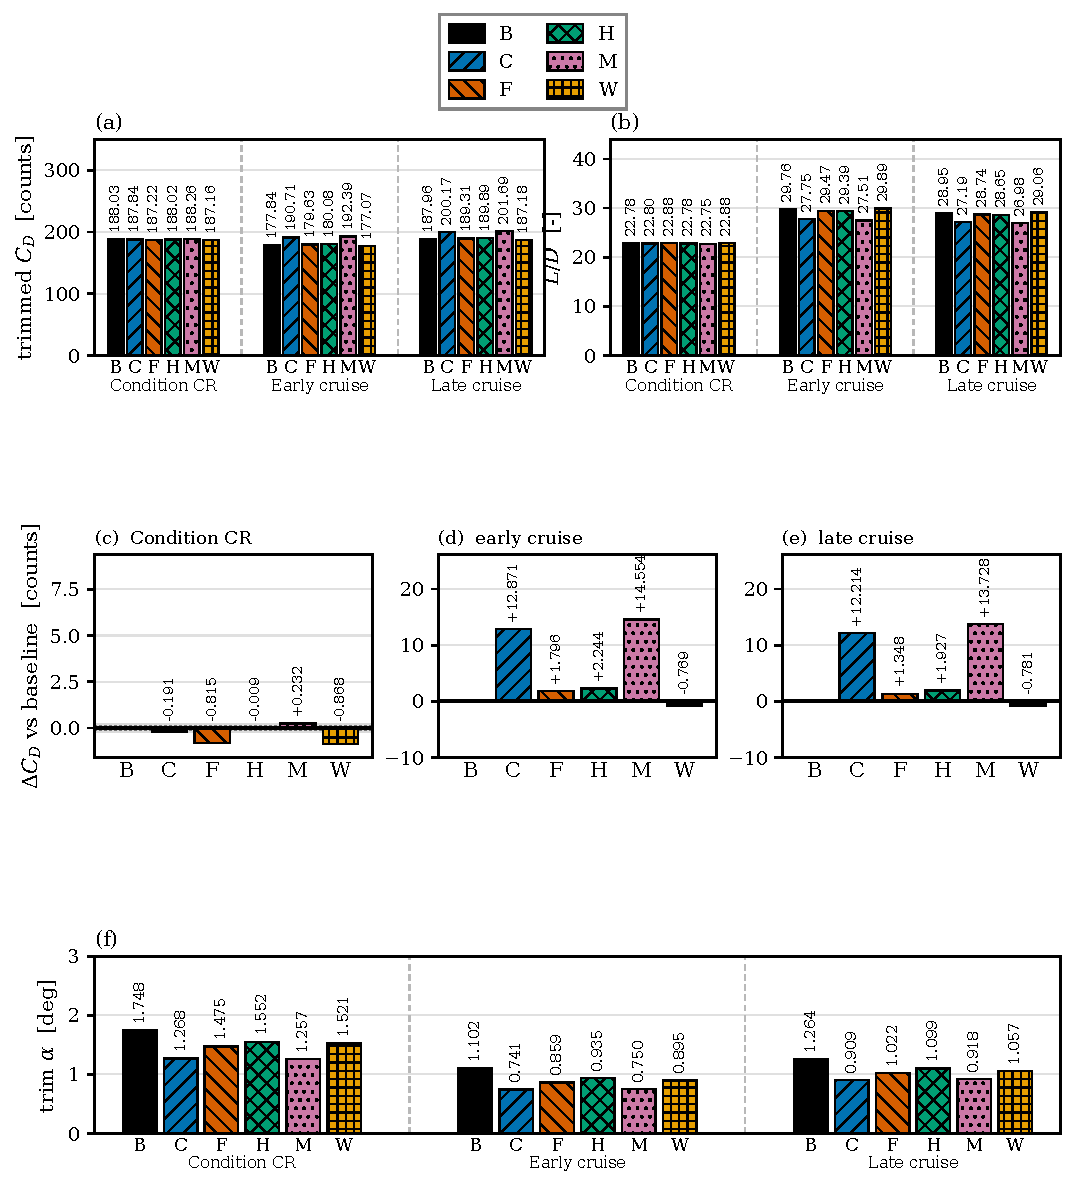
\includegraphics[width=\linewidth]{fig/fig_trimmed_performance.pdf}
\caption{Trimmed performance at matched lift, all six geometries, all three conditions. Panels:
(a) trimmed $C_D$, (b) $L/D$, (c) $\Delta C_D$ at Condition CR, (d) $\Delta C_D$ at early cruise,
(e) $\Delta C_D$ at late cruise, and (f) trim incidence. (d) and (e) share one vertical scale;
Condition CR keeps its own or its deltas would be invisible. Every delta is formed inside one
condition against that condition's own B trim. DSO basis, half model,
$A_\mathrm{ref}=\num{0.620462}$~m$^2$. Source: \texttt{data/rans\_forces.json}.}
\label{fig:perf:trimmed}
\end{figure}

\subsubsection{Why the cruise penalty appears, and why W escapes it}
\label{sec:perf:mechanism}
\textbf{Mechanism.} At $M = 0.78$ the upper surface at $\eta = 0.80$ is supersonic over most of
the chord on every geometry, $144$ to $153$ of $200$ chordwise bins below
$c_p^{*}=-0.4931$ at early cruise. What separates the candidates is how that supersonic region
ends. On B and W it recompresses without a shock: the steepest gradient is
$\mathrm{d}c_p/\mathrm{d}(x/c) = 4.22$ and $4.53$, both at $x/c = 0.8725$, below the shock
threshold of $15$. F and H end it in a moderate shock, $17.1$ at $x/c = 0.7525$ and $19.1$ at
$0.7725$, and stay attached. C and M end it in a strong shock, $45.7$ at $0.7375$ and $50.7$ at
$0.7275$, and separate behind it. \textbf{The drag ordering follows the shock strength}: W within
a count of the baseline, F and H about two counts above it, C and M twelve to fifteen. Late cruise
repeats the pattern at slightly lower strength, $16.1$ and $16.8$ on F and H and $43.6$ and
$38.0$ on C and M. At $M=0.10$ the same camber meets subsonic flow and the field stays inside a
count and a half.

\textbf{Where the load moves.} Figures~\ref{fig:perf:loading} and~\ref{fig:perf:loading:lc} show
the redistribution. Every candidate unloads the inboard wing and loads the outboard wing; the
difference from B crosses zero between $\eta = 0.571$ and $0.652$ and peaks between $0.725$ and
$0.800$, at the same stations to three decimals at both cruise points. The inboard and outboard
integrals cancel, as they must at fixed lift. C and M carry the largest outboard increment,
$+0.075$ and $+0.077$ in $c_l c/C_\mathrm{ref}$ at early cruise, against $+0.046$ for F, H and W,
and that peak sits under the outboard shock.

\textbf{Separation.} Two bands separate in the 30 sampled at each cruise point, and they are the
same two: \texttt{CMPC\_trim} and \texttt{CMPM\_trim} at $\eta = 0.80$
(Figure~\ref{fig:perf:shock}), and their late-cruise counterparts. Reversed flow covers
$23.3$~per~cent of C's upper-surface faces in that band at early cruise, from $x/c = 0.743$ to
$0.992$, and $23.9$~per~cent of M's, from $0.730$ to $0.997$; at late cruise the figures are
$24.1$ and $25.3$~per~cent. Every other cruise band reverses at most $0.019$~per~cent of its
upper-surface faces, and nothing separates at Condition~CR. The cases are wall modelled, so the
sign of this result is firm and its extent carries the precision of the section cuts. The strong
shock and the separation occur together, on the two strong-camber candidates, and they are the
two most expensive. Appendix~\ref{sec:app:sections:ec} gives the station detail.

\begin{figure}[htbp]
\centering
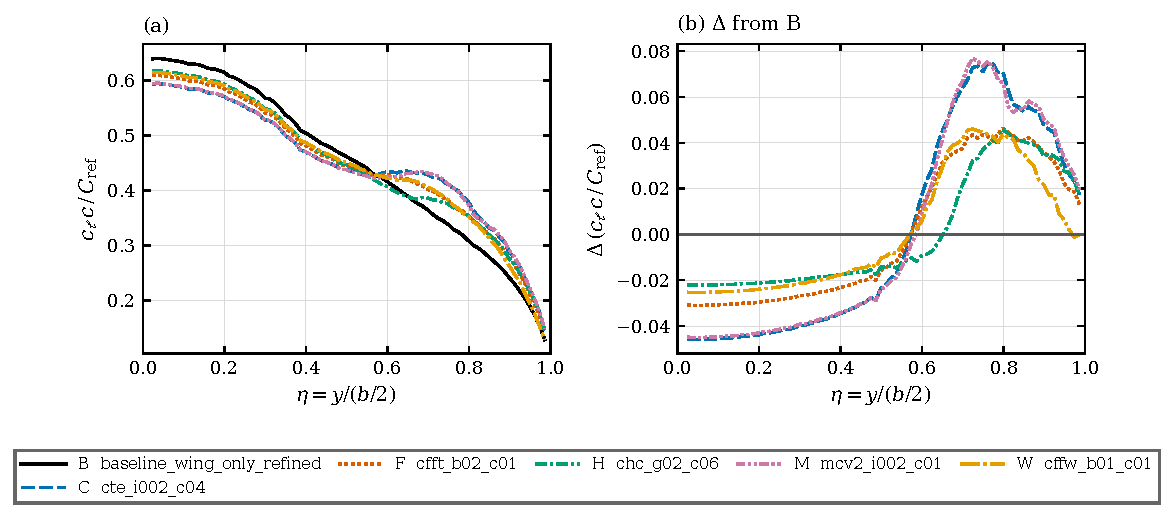
\includegraphics[width=0.46\linewidth]{fig/spanwise_loading_early_cruise.pdf}
\caption{Spanwise loading at early cruise, $M=0.78$, every case trimmed to
$C_L=0.529297087450$. Sectional load $c_l c/C_\mathrm{ref}$ against $\eta$, and the difference
from \texttt{CMPB\_trim}, over 78 stations. Sectional $c_l$ is pressure only. DSO basis,
$C_\mathrm{ref}=\num{0.39396}$~m.}
\label{fig:perf:loading}
\end{figure}

\begin{figure}[htbp]
\centering
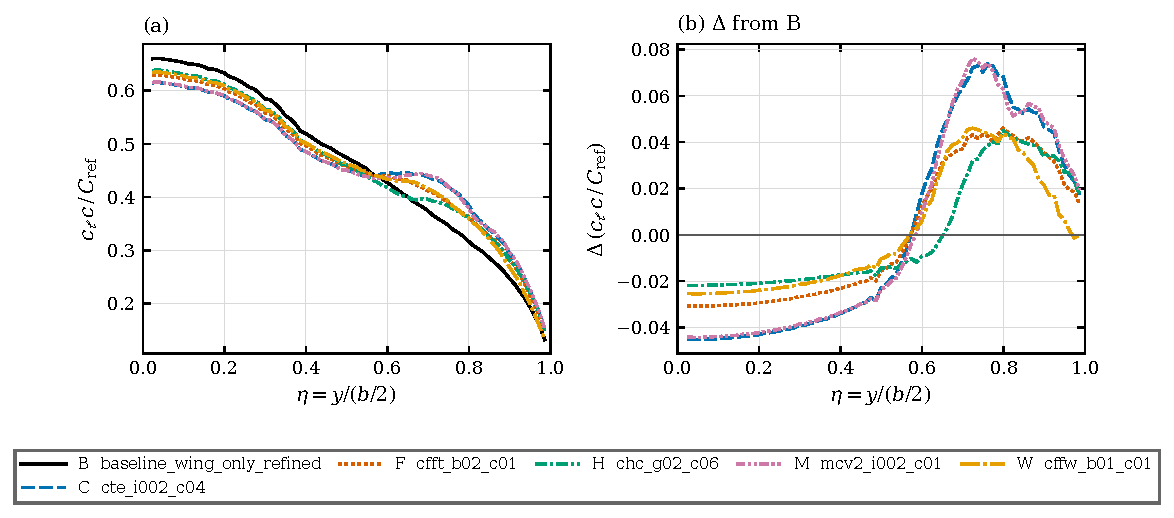
\includegraphics[width=0.46\linewidth]{fig/spanwise_loading_late_cruise.pdf}
\caption{Spanwise loading at late cruise, $M=0.78$, $C_L=0.544114800210$, against
\texttt{LCB\_trim}. As Figure~\ref{fig:perf:loading}.}
\label{fig:perf:loading:lc}
\end{figure}

\begin{figure}[htbp]
\centering
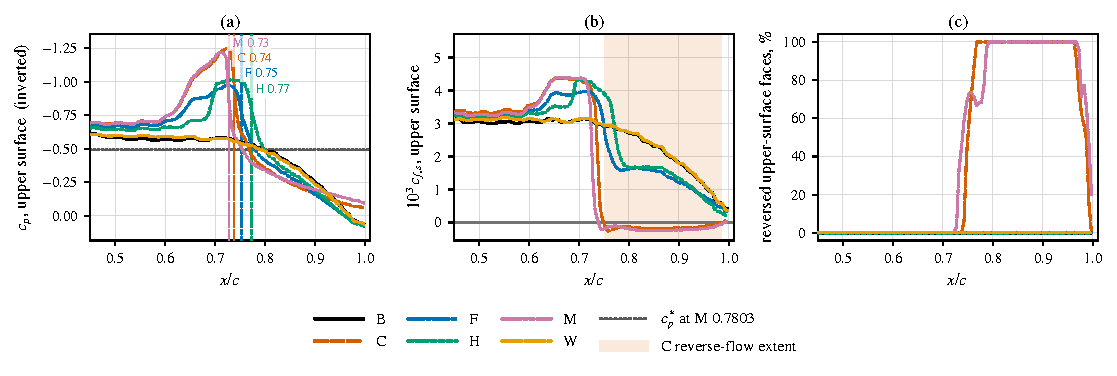
\includegraphics[width=0.46\linewidth]{fig/fig_cp_shock_separation_CMPC.pdf}
\caption{One of the two separated bands: \texttt{CMPC\_trim} at early cruise, $\eta=0.80$.
Upper-surface $c_p$, signed freestream-aligned skin friction and reverse-flow fraction. The shock
sits at $x/c=0.7375$ with $\Delta c_p=0.724$ and $c_p=-1.154$ upstream, against
$c_p^{*}=-0.4931$. \texttt{CMPM\_trim} separates at the same station and is drawn beside C in
Figure~\ref{fig:perf:cp:ec}. $c_p$ and $c_f$ carry no reference area.}
\label{fig:perf:shock}
\end{figure}

Section pressure and skin friction at the five spanwise stations, at Condition~CR and both cruise
points, are in Appendix~\ref{sec:app:sections}.

\subsection{Trim angle}
\label{sec:results:trim}
\label{sec:qv:lift}
\textbf{Result.} Trim angle is where the two methods agree best (Table~\ref{tab:qv:lift},
Figure~\ref{fig:qv:trimalpha}). VSPAERO matches the solved RANS angle to within
$0.105^{\circ}$ on all five candidates, and to $0.016^{\circ}$ or better on three of them.
Carried through each family's own fitted lift slope, that is a lift error of at most
2.13~per~cent of the target $C_L$. The baseline B is the outlier at $+0.252^{\circ}$, and its deck
is the only Condition CR run to miss its own target, by $1.53\times10^{-5}$ in $C_L$.

\textbf{Slope.} The RANS side fits $\mathrm{d}C_L/\mathrm{d}\alpha = 0.0860$ to $0.0870$ per
degree over 4 or 5 solved angles per family, with residuals of $1.6\times10^{-4}$ to
$1.1\times10^{-3}$ in $C_l$. The decks are single-point, so the VLM side carries no lift slope and
the comparison is made on trim angle, which needs no derivative.

\begin{table}[htbp]
  \centering
  \footnotesize
  \caption{Trim angle at the common Condition CR target $C_L = 0.428277635108$, both sides on the
  DSO basis, conversion factor exactly 1.000000. RANS $\alpha$ comes from the solved trim case's
  own \texttt{dragDir} header. Implied $\Delta C_L$ is $\Delta\alpha$ through that family's own
  fitted RANS slope, as a percentage of the target. \textbf{Each slope is fitted over that
  family's published alpha-sweep legs together with its Condition~CR trim case, and the trim
  case alone was solved again on the rebuilt mesh: each slope is therefore fitted over legs
  from two different meshes and is not a single-mesh derivative.} They enter only $\Delta\alpha$ converted to
  an implied $\Delta C_L$, which is at most $2.13$ per cent of target, and no drag number in
  this report is formed through them. Rows generated by
  \texttt{scripts/make\_rank\_table.py} from \texttt{fig/fig\_vlmerr\_values.json}.}
  \label{tab:qv:lift}
  \begin{tabular}{lrrrrr}
    \toprule
    Geom. & $\alpha_\mathrm{RANS}$ [deg] & $\alpha_\mathrm{VLM}$ [deg] & $\Delta\alpha$ [deg] & implied $\Delta C_L$ [\%] & $\mathrm{d}C_L/\mathrm{d}\alpha$ [/deg] \\
    \midrule
    B & 1.747609 & 1.99981 & $+0.2522$ & $+5.06$ & 0.085980 \\
    C & 1.268311 & 1.25652 & $-0.0118$ & $-0.24$ & 0.086042 \\
    M & 1.257423 & 1.24972 & $-0.0077$ & $-0.15$ & 0.086119 \\
    F & 1.475456 & 1.45936 & $-0.0161$ & $-0.33$ & 0.087035 \\
    W & 1.520545 & 1.42193 & $-0.0986$ & $-1.99$ & 0.086510 \\
    H & 1.552310 & 1.44697 & $-0.1053$ & $-2.13$ & 0.086784 \\
    \bottomrule
  \end{tabular}
\end{table}

\subsection{Spanwise load}
\label{sec:cr:loads}
\textbf{Result.} Figure~\ref{fig:geom:spanwise} shows the sectional load defined in
Section~\ref{sec:qv:qoi} for every geometry at its trim, with the VSPAERO loading beside it. The
absolute curves lie on top of one another and show the planform. The difference from baseline
isolates the morphing, and it sits over the morphed span in every case; how closely the two
methods agree on that redistribution is Section~\ref{sec:qv:span}.
\begin{figure}[htbp]
  \centering
  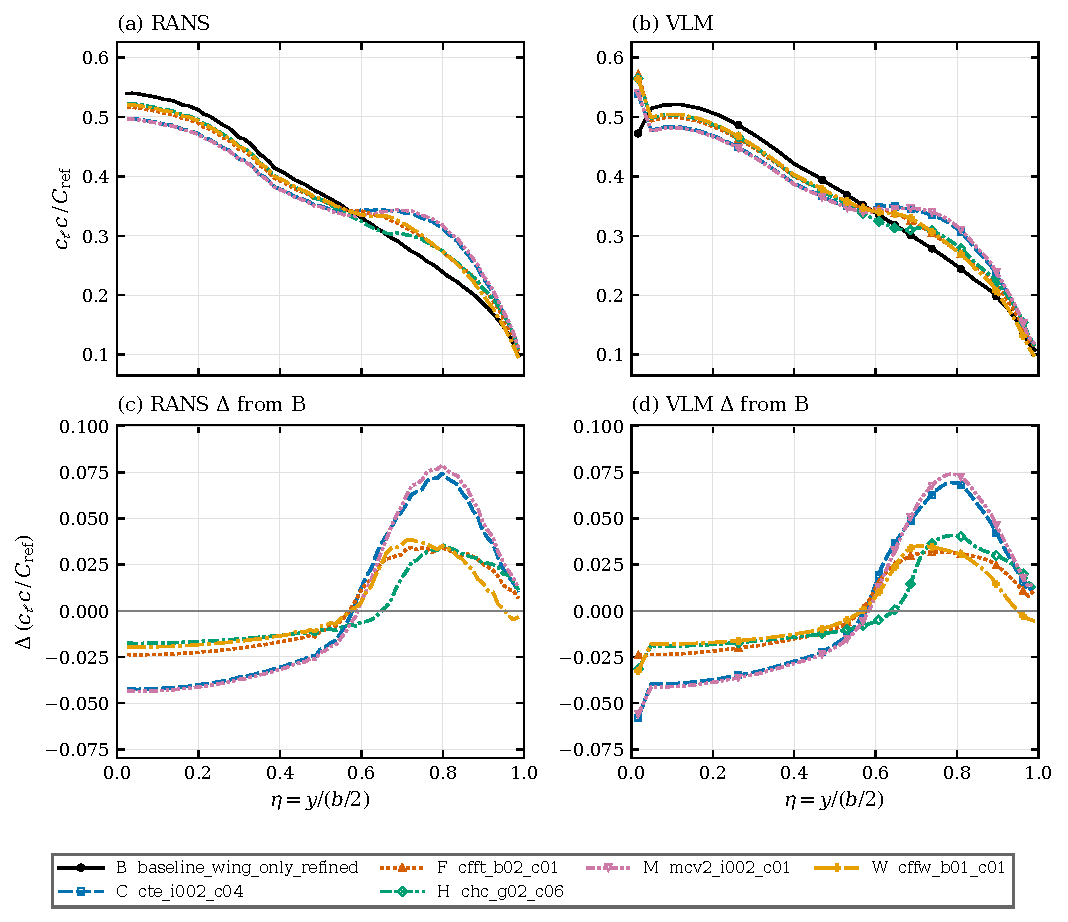
\includegraphics[width=0.94\linewidth]{fig/spanwise_loading_condition_CR.pdf}
  \caption{Spanwise loading at Condition~CR, $M = 0.10$, every geometry trimmed to
  $C_L = 0.428277635108$ on the DSO basis. The upper row is the sectional load
  $c_l c / C_\mathrm{ref}$ against $\eta$, where the six geometries differ by a few per~cent and
  the curves overlie. The lower row is each candidate minus the baseline of the same method,
  which is where the morphing appears. The RANS difference peaks at $\eta = 0.7985$ for C, F, H
  and M, and at $\eta = 0.7237$ for W, the one candidate whose command peaks furthest inboard.
  Peak differences are $0.079$ (M), $0.075$ (C), $0.040$ (W), $0.037$ (H) and $0.036$ (F). RANS
  curves carry 78 dense stations over $\eta = 0.025$ to $0.986$; VSPAERO curves carry 69 strips.
  Generated by \texttt{fig/make\_spanwise.py} from \texttt{data/spanwise/} and
  \texttt{data/vlm.json}.}
  \label{fig:geom:spanwise}
\end{figure}

\label{sec:qv:span}

\textbf{Result.} The VLM puts the load where the RANS puts it (Figure~\ref{fig:geom:spanwise}).
Each side is differenced against its own baseline, which is the quantity the optimiser acts on.
Over 78 stations the difference between the two redistributions has an r.m.s.\ of 0.0015 to
0.0037 in $c_l c/C_\mathrm{ref}$, against RANS peaks of 0.034 to 0.080. That is 4.5 to
9.5~per~cent of the peak. The station of peak change agrees to within 0.049 in $\eta$, and to
within 0.014 on four of the five candidates.
\textbf{Resolution.} The RANS gives 78 stations and the VLM 69 strips, interpolated onto a common
grid with an error bound of $8.5\times10^{-4}$. The VLM strips close to their own polar $C_L$ to
$4.6\times10^{-6}$ once the half-wing factor of two is applied, and to 50.0~per~cent without it.
The RANS loading is integrated from the wing surface, pressure only; the VLM loading comes from
the 69 strips of each deck's own \texttt{.lod}. Both are on $C_\mathrm{ref} = 0.39396$~m, the DSO
basis.

\subsection{Induced drag and span efficiency}
\label{sec:cr:spaneff}
\label{sec:spaneff}
\textbf{Method.} Induced drag is taken from the crossflow kinetic energy crossing four
transverse planes in the wake, at $x = 2.394$, $2.626$, $2.916$ and $3.206$~m, sampled by a
function object inside the solver rather than reconstructed afterwards. Span efficiency
follows from it as
%
\begin{equation}
  e \;=\; \frac{C_L^{2}}{\pi \, AR \, C_{Di}} ,
  \label{eq:spaneff}
\end{equation}
%
with $AR$ the full-wing aspect ratio on the DSO basis. Every geometry is evaluated at its
own trimmed angle of attack, and the freestream component is removed using that case's own
$\alpha$; using a different one would leave a uniform residual across the whole plane.

\textbf{Frame.} $C_{Di}$ is on the half wing, $A_\mathrm{ref} = 0.620462$~m$^2$, matching
each case's own force coefficients. $e$ is on the full-wing aspect ratio from the DSO basis,
$b_\mathrm{ref} = 3.6576$~m and $S_\mathrm{ref} = 1.24092$~m$^2$. Condition~CR,
$U_\infty = 34.0$~m/s, every geometry trimmed to $C_L = 0.428277635108$.

\textbf{There is no plateau, so the spread is the uncertainty.} Crossflow kinetic energy is
conserved in an inviscid wake, so a Trefftz integral should not decay downstream at all.
What decay remains is numerical: the grid dissipating the trailing vortex system between one
plane and the next. Quoting a single station would therefore report a number without the
quantity that qualifies it, and Figure~\ref{fig:spaneff} plots all four.

\textbf{The limit at $e = 1$ is a check, not a target.}
For a planar wake $e = 1$ is the elliptical optimum and cannot be exceeded. That makes it
useful twice over: as the reference a spanload is measured against, and as a check on the
calculation itself. A value above~1 would report less induced drag than the theoretical
minimum, which is not a marginal result to be discussed but an arithmetic impossibility, so
any geometry returning one is withheld rather than plotted. Every value in
Figure~\ref{fig:spaneff} sits below the line, as it must.

% RESULT PARAGRAPH: generated. Run
%     python3 fig/make_spaneff.py
%     python3 scripts/spaneff_prose_values.py
% and paste what the second prints. Do NOT hand-write these figures: the decay percentages
% and e values move with every re-trim, and this section is the one place in the report
% where a stale e could be mistaken for a physical result rather than a numerical one.
\textbf{Result.} Span efficiency at the last station ranges from $0.9673$ on the rigid baseline B to $0.9859$ on F, every value below the planar-wake limit. Induced drag at that station spans $54.93$ to $55.98$ counts.

\textbf{Decay between the first and last plane} is $9.5$ to $10.2$ per cent, and is consistent across the geometries: B $9.46$\,\%, W $9.68$\,\%, F $9.95$\,\%, H $9.98$\,\%, C $10.19$\,\%, M $10.22$\,\%. That consistency matters more than the magnitude, because a decay rate that differed between geometries would mean the comparison was being made on wakes resolved to different degrees, and no difference between them could be attributed to the wing.

\textbf{Against the baseline.} Every candidate measured here carries a higher span efficiency than the rigid baseline's $0.9673$ (C, F, H, M and W). The margin is small, one to two per cent, which is the size of spanload improvement the low-order design study predicted for this class of change.


\begin{figure}[htbp]
  \centering
  \includegraphics[width=\linewidth]{fig_spaneff.pdf}
  \caption{Trefftz-plane induced drag and the span efficiency it implies, Condition~CR,
  $M = 0.10$, every geometry trimmed to $C_L = 0.428277635108$. Panel~(a) is $C_{Di}$ at
  each of the four sampled stations; panel~(b) is $e$ from
  Equation~\ref{eq:spaneff}, with the planar-wake limit $e = 1$ marked. $C_{Di}$ is on the
  half wing, $A_\mathrm{ref} = 0.620462$~m$^2$; $e$ is on the DSO-basis full-wing aspect
  ratio. Generated by \texttt{fig/make\_spaneff.py} from
  \texttt{data/span\_efficiency.json}, which is assembled by
  \texttt{scripts/build\_span\_efficiency.py}, which refuses to mix meshes, to mix
  untrimmed legs with trimmed ones, or to carry a value above the physical limit.}
  \label{fig:spaneff}
\end{figure}

\textbf{Span efficiency.} The two methods agree on the level once the far-field definition is
used. VSPAERO reports $E_w = 0.960$ to $0.972$ on the five candidates against its own near-field
$E = 0.568$ to $0.587$, and the RANS Trefftz integral returns $0.972$ to $0.986$ on the
five candidates. The near-field $E$ is not a competing estimate of
the same quantity; it is the one that produced the sign violation reported in
Section~\ref{sec:qv:vlmmethod}.

\subsection{Hinge moment about the morph line}
\label{sec:loads}
\label{sec:hinge}
\textbf{Purpose.} Two structural quantities bear on the concept selection. The hinge moment about
the morph line is the load the actuator reacts, and the low-order method cannot produce it. Root
bending is the active screen the design study selected on, and the low-order method does produce
it, so it is the one structural quantity where the two methods compare directly. Both are reported
here for every geometry at every operating point that carries them.

\textbf{Purpose.} This section reports the aerodynamic moment the actuator has to react. It is
the one quantity in this campaign that the low-order method cannot produce at all: the DSO's own
per-case summary records \texttt{hinge\_moment\_status} as
\texttt{not\_computed\_requires\_surface\_pressure\_integration} for every one of its 23 runs, so
there is no VLM column to compare against and none is constructed here. The decks do carry a
$C_{My}$, but that is the whole-model pitching moment about the deck's own reference point, a
different quantity in a different frame, and reaching a hinge moment from it needs a transfer
formula this project refuses (\texttt{scripts/hinge\_moment.py}).

\textbf{Definition, as agreed with the DSO team.} Every element below is the agreed form and none
of it is a local choice.

\begin{enumerate}
  \item \textbf{Axis:} the swept spanwise line through $x_h/c = 0.62$ at each local section, with
    the moment projected on that line's \emph{local tangent}. The line is swept and tapered, so
    its tangent is not the $y$ axis and projecting on $y$ instead is the error a careful reader
    makes first.
  \item \textbf{Sign:} positive is trailing-edge down. The actuator reaction is the opposite sign.
  \item \textbf{Scope:} surfaces aft of the line only, over $0.60 \leq \eta \leq 1.00$, half wing.
    Aft-of-line is tested per station against $x_h$ at each face's own $y$, never against a single
    global $x$ cut, which on a swept wing would include forward surface at the root and exclude
    aft surface at the tip.
  \item \textbf{Sectional:} $m'_h$ in N\,m/m and $c_{mh} = m'_h/(q_\infty c(y)^2)$ on the
    \emph{local} section chord, because this wing has several defensible reference chords.
  \item \textbf{Integrated:} $M_h$ in N\,m and
    $C_{Mh,\mathrm{region}} = M_h/[q_\infty\!\int\! c(y)^2\,\mathrm{d}y]$ over the same region,
    which avoids selecting one of them.
  \item \textbf{Terms:} pressure is the primary result, the viscous term is reported separately,
    and the total is given.
\end{enumerate}

\textbf{Result.} Table~\ref{tab:hinge} gives every geometry at every condition that carries a
solved trim. \textbf{Every candidate raises the hinge moment above the rigid baseline, at all
three operating points, without exception.} The increase is $2.0$ to $5.0$~per~cent at Condition~CR,
$0.5$ to $6.3$~per~cent at early cruise and $0.4$ to $6.2$~per~cent at late cruise. H is the
largest at every condition, which is what a discrete hinged surface should do: it turns a rigid
segment against the flow rather than redistributing camber smoothly. W is the smallest at both
cruise points.

\textbf{The ordering is preserved between the conditions, up to one near-tie.} From largest
magnitude to smallest it is H, M, C, F, W, B at both cruise points and H, M, C, W, F, B at
Condition~CR, where W and F differ by $0.0006$~N\,m, $0.07$~per~cent of the baseline moment. A
hinge moment measured at low speed therefore ranks the candidates for cruise, as the drag does
(Section~\ref{sec:perf:inversion}).

\textbf{Both orderings rank the candidates on the common comparison line, not on the load each
concept's own actuator carries.} For C, F and M those are the same thing; for H and W they are
not, and W's differs in region as well as in axis. Section~\ref{sec:hinge:hcaveat} states which
rows are actuator moments and which are comparisons only. Read it before using any row to size
a mechanism or to rank the concepts against one another on actuator load.

\textbf{The viscous term is small and it is reported, not assumed.} It runs $0.37$ to
$0.44$~per~cent of the total at Condition~CR and $0.13$ to $0.17$~per~cent at cruise. It is
computed from the sampled wall-shear vector, whose sign convention is measured rather than
inferred: OpenFOAM's \texttt{wallShearStress} is the negative of the traction on the body, and a
wall shear that integrates to a thrust along the freestream is refused outright.

\begin{table}[htbp]
  \centering
  \footnotesize
  \caption{Hinge moment at trim, every geometry and condition, all integrated about the common
  comparison line $x_h/c = 0.62$ over $0.60 \leq \eta \leq 1.00$. $\Delta$ is against that
  condition's own baseline B. \textbf{The last column is load-bearing: only the rows marked
  ``yes'' are the moment that concept's own actuator reacts.} (a) H's hinge is at $x/c = 0.70$,
  so the strip from $0.62$ to $0.70$ lies forward of it and is inside this integral but outside
  H's actuator load. (b) W rotates the whole section about $x/c = 0.25$, so its actuator reacts a
  \emph{torsional} moment over the entire section rather than a hinge moment about $0.62$ over the
  aft $38$ per cent; that quantity is not computed in this campaign. Rows (a) and (b) are valid
  comparisons on a shared line and must not be used to size a mechanism or to rank concepts on
  actuator load. Source: \texttt{fig/hinge\_moment\_values.csv},
  rows generated by \texttt{scripts/make\_cruise\_tables.py}.}
  \label{tab:hinge}
  \begin{tabular}{llrrrrrl}
    \toprule
    & Geometry & $M_h$ [N\,m] & $\Delta M_h$ & $\Delta$ \% & $C_{Mh,\mathrm{region}}$ &
      visc.\ \% & actuator? \\
    \midrule
\inputrows{sections/gen/tab_hinge_rows.tex}
    \bottomrule
  \end{tabular}
\end{table}

\textbf{Reading the two figures.} Both carry one panel per condition, and in both the upper row is
\emph{dimensional} while the lower row is the coefficient. The three conditions sit at
$q = 708.05$, $\num{11292.80}$ and $\num{8257.37}$~Pa, so an $M_h$ or an $m'_h$ from one panel may
not be read against another; $C_{Mh,\mathrm{region}}$ and $c_{mh}$ may, which is why both rows are
drawn. Sectional loading falls monotonically outboard in every case, following the chord, and the
candidates separate from the baseline over the commanded span.

\textbf{The sectional lines are smoothed for display and the integral is not smoothed at all.}
The curves carry a Hann average over $8$~per~cent of the band. What it removes is an artefact of
the reporting bins rather than a feature of the flow: the raw values alternate from station to
station at a lag-one autocorrelation of $-0.49$ on all three baselines, and a block rebin to $91$
stations left that at $-0.49$ while shrinking only the amplitude, which is what established it is
not a physical oscillation. Smoothing moves it to $+0.89$ and takes the direction reversals from
$427$ to $1$, leaving the distribution's shape untouched. The unsmoothed stations are kept in the
per-case records under \texttt{results/derived/}. Nothing is smoothed before integration: $M_h$ in
Table~\ref{tab:hinge} is a direct sum over faces and never passes through these stations.

\begin{figure}[htbp]
  \centering
  \includegraphics[width=\linewidth]{fig_hinge_sections.pdf}
  \caption{Sectional hinge moment against $\eta$. Upper row $m'_h$, lower row $c_{mh}$ on the
  local chord. Lines are smoothed for display.}
  \label{fig:hinge:sections}
\end{figure}

\begin{figure}[htbp]
  \centering
  \includegraphics[width=\linewidth]{fig_hinge_integrated.pdf}
  \caption{Integrated hinge moment, half wing. Upper row $M_h$, lower row
  $C_{Mh,\mathrm{region}}$. The printed value is the total; the viscous share is annotated.}
  \label{fig:hinge:integrated}
\end{figure}

\subsubsection{Which of these numbers are actuator moments, and which are only comparisons}
\label{sec:hinge:hcaveat}

All six geometries are integrated about $0.62$ because the agreed definition fixes one common
comparison line, and $C_{Mh,\mathrm{region}}$ means nothing unless all six share it. That makes
every number in Table~\ref{tab:hinge} a valid \emph{comparison} on a common basis. It does not make
all of them actuator moments, and the distinction is not cosmetic for anyone sizing a mechanism.

\textbf{Three of the five morphed candidates act on the line integrated about.} C, F and M are
continuous trailing-edge camber: the morph starts at $x/c = 0.62$, the surface aft of that line is
the surface that moves, and the moment reported is the moment their actuator reacts.

\textbf{H's own hinge is not at $x_h/c = 0.62$.} It is at $0.70$ (Section~\ref{sec:geom:law}). The
strip between $x/c = 0.62$ and $0.70$ lies \emph{forward} of its real hinge, so it is inside the
integral reported here and outside the load H's own actuator carries. H's number is therefore
correct as a comparison and is not H's actuator moment.

\textbf{W is not a hinged concept at all, and its row is the one most easily misread.} Distributed
twist rotates the whole local section about $x/c = 0.25$, and it is the one candidate whose leading
edge moves (Section~\ref{sec:geom:law}). Its actuator reacts a \emph{torsional} moment, taken about
the quarter chord and over the \emph{entire} section, whereas the quantity tabulated here is taken
about $0.62$ and over the aft $38$~per~cent only. The axis is displaced by $0.37c$ rather than H's
$0.08c$, and the region of integration is wrong as well as the line. \textbf{W's number is a
common-basis comparison and is not, even approximately, W's actuator moment.} The torsional moment
about $x/c = 0.25$ has not been computed in this campaign; it is the same integral over a different
region about a different line, and it is the number the structures and actuator group needs before
distributed twist can be sized or ranked against trailing-edge morphing on actuator load.

\subsubsection{Method uncertainty, measured}
\label{sec:hinge:uncertainty}

\textbf{The spanwise resolution is not free, and it was quantified rather than chosen.} The hinge
line is built from a planform binned in $y$, and the local chord is taken as the extreme $x$ within
each bin, so a coarse bin overstates the chord, moves $x_h = x_\mathrm{LE} + 0.62c$ against the
surface, and changes which faces count as aft of the line. Sweeping the bin count on
\texttt{SWB\_trim} gives $M_h = 0.9375$, $0.8972$, $0.8774$, $0.8677$ and $0.8630$~N\,m at
$100$, $200$, $400$, $800$ and $1600$ bins, with the selected face count falling from
$\num{523627}$ to $\num{501559}$ and the mean chord from $0.2217$ to $0.2135$~m while the mean
$x_h$ holds to $0.015$~per~cent. The increments halve on each doubling, so the convergence is
first order and Richardson puts the limit near $0.858$~N\,m.

\textbf{Every number in this section is at 1600 bins}, which sits about $0.5$~per~cent from that
limit, and $0.5$~per~cent is the figure to quote as the method uncertainty on an absolute $M_h$.
The module's default of 200 bins was $4.5$~per~cent high in magnitude and is superseded. The
\emph{orderings} are unaffected: both condition orderings are identical at 200 and at 1600 bins,
so the ranking was robust to a bias the magnitudes were not.

\textbf{Late cruise.} All eighteen condition-by-geometry cells are integrated, so the third
operating point carries its full six-way comparison. Every candidate raises the magnitude of the
moment about the common line, by $0.4$~per~cent on W to $6.2$~per~cent on H, the same direction
and nearly the same size as at early cruise, and the ordering is identical at the two cruise
points. The actuator-load comparison between these concepts therefore does not depend on which
cruise condition is chosen.

\subsection{Root bending, against the low-order method and against its screen}
\label{sec:rbm}
\textbf{Purpose.} Root bending is one of the two inequality screens the design study selected
on, and the study's own report calls it \emph{the active screen} for the low-speed selection.
Unlike the hinge moment of Section~\ref{sec:hinge}, the low-order method \emph{does} produce it,
so this is the one structural quantity where the two methods can be compared directly. This
section asks two things: do they agree, and does the viscous answer still satisfy the screen.

\textbf{What is compared, and on which basis.} The RANS value is the half-wing moment about the
root chord line, taken from each case's own solver moment output about a centre of rotation
asserted to lie on the symmetry plane. It is not integrated from a surface: root bending needs no
chordwise resolution, so the solver's own $M_x$ is both the more direct route and the one
available for every case. The VLM value is the half-wing root bending in each delivered
optimisation record.

\textbf{Two normalisations have to be stated or the comparison is meaningless.} First, \textbf{root
bending is dimensional}. The VLM decks run at $100$~ft/s and this campaign at $34$~m/s, which is
$q = 569.03$ against $708.05$~Pa, a ratio of $1.24431$. Comparing the two moments without that
factor is wrong by $24$~per~cent before any physics enters. Second, \textbf{the two percentages
are against different baselines}: the VLM differences are against the corrected-interpolation
baseline B$^{*}$, whose own record states it sits $-1.67$~per~cent from the original, while the
RANS differences are against B, the surface that was actually meshed and solved. The percentage
is the primary comparison because it cancels $q$; the dimensional column is reported beside it
precisely because a baseline disagreement would otherwise hide inside the percentages.

\textbf{Result: the two methods agree to better than half a percentage point.}
Table~\ref{tab:rbm} gives both. Every candidate agrees within $0.40$ percentage points, and after
the $q$ ratio the dimensional moments agree to between $0.12$ and $0.88$~per~cent. That is far
closer than the drag comparison of Section~\ref{sec:qv:counts}, and the reason is physical: root
bending is the first moment of the spanwise lift distribution, which a vortex-lattice method
resolves well, and viscosity contributes very little to it. The lift centroid moves outboard with
the morphing exactly as the moment does, from $\eta = 0.3985$ on the baseline to $0.4286$ on M.

\textbf{Result: the viscous calculation breaks the screen on C.} The screen is a $6.8$~per~cent
increase over the rigid baseline. C is the design study's strict optimum and sits at
$+6.796$~per~cent in the VLM, which is $99.94$~per~cent of the screen: the study's own report
says the optimum ``lies immediately below'' it. \textbf{The RANS puts C at $+7.170$~per~cent,
which is over.} M was already over in the low-order method, at $+7.124$, and the RANS agrees and
puts it further over at $+7.519$. F, H and W are comfortably inside on both methods.

\textbf{What that does and does not mean.} The design study states the $6.8$~per~cent figure is
``a study-level bound rather than a certified structural limit'', and that its root bending is
approximated. So this is a flag for the structures and actuator group, not a failure against a
certified allowable. What it does establish is that the constraint which \emph{selected} C is not
satisfied once the same quantity is computed viscously, and that the margin it was selected on,
$0.004$ percentage points, was far smaller than the $0.37$ percentage point difference between the
two methods.

\begin{table}[htbp]
  \centering
  \footnotesize
  \caption{Half-wing root bending at Condition~CR. VLM percentages are against B$^{*}$, RANS
  against B. ``VLM$\times$ratio'' scales the VLM moment by $q_\mathrm{RANS}/q_\mathrm{VLM} =
  1.24431$. Source: \texttt{fig/rootbending\_values.csv}.}
  \label{tab:rbm}
  \begin{tabular}{llrrrrrr}
    \toprule
    & Geometry & VLM \% & RANS \% & diff (pp) & VLM$\times$ratio & RANS [N\,m] & dim.\ \% \\
    \midrule
    B & baseline & $+0.000$ & $+0.000$ & $+0.00$ & $137.805$ & $137.133$ & $+0.49$ \\
    C & \texttt{cte\_i002\_c04}  & $+6.796$ & $\mathbf{+7.170}$ & $+0.37$ & $147.171$ & $146.965$ & $+0.14$ \\
    F & \texttt{cfft\_b02\_c01}  & $+3.755$ & $+3.960$ & $+0.20$ & $142.980$ & $142.563$ & $+0.29$ \\
    H & \texttt{chc\_g02\_c06}   & $+3.769$ & $+3.368$ & $-0.40$ & $142.999$ & $141.752$ & $+0.88$ \\
    M & \texttt{mcv2\_i002\_c01} & $+7.124$ & $\mathbf{+7.519}$ & $+0.40$ & $147.623$ & $147.444$ & $+0.12$ \\
    W & \texttt{cffw\_b01\_c01}  & $+3.010$ & $+3.079$ & $+0.07$ & $141.953$ & $141.355$ & $+0.42$ \\
    \bottomrule
  \end{tabular}
\end{table}

\begin{figure}[htbp]
  \centering
  \includegraphics[width=\linewidth]{fig_rootbending.pdf}
  \caption{Root bending increase against each method's own baseline, with the $6.8$~per~cent
  screen; and the dimensional agreement after the $q$ ratio.}
  \label{fig:rbm}
\end{figure}

\subsubsection{One delivered percentage is stale, and it is the one that matters}
\label{sec:rbm:stale}

\textbf{M's delivered increase is wrong in the file.} \texttt{mcv2\_i002\_c01} records a moment of
$118.64405$~N\,m and an increase of $5.3352$~per~cent. Those two are inconsistent:
$118.64405 / 110.75354 = 1.07124$, an increase of $7.124$~per~cent. The moment is the corrected
value while the percentage was formed against the pre-correction baseline. The design study's own
report states the correct figure in prose, ``the unchanged candidate now increases half-wing root
bending by $7.12$~per~cent, above the illustrative $6.8$~per~cent screen'', so this is a known
defect in the delivered record rather than a new disagreement. \textbf{Every percentage in
Table~\ref{tab:rbm} is recomputed from the two moments rather than read}, and the generator
carries the delivered value alongside and flags the disagreement, so the discrepancy is visible
rather than silently corrected. A reader taking the number straight from the CSV would conclude M
passes the screen by $1.5$ percentage points when it fails it by $0.3$.

\subsubsection{Cruise, and why there is no low-order column}
\label{sec:rbm:cruise}

\textbf{The five candidates do not appear in the study's cruise set at all.} That set contains
optimiser seeds and the rigid baseline, indexed by concept rather than by the geometries meshed
here, so there is no VLM root bending to compare against at either cruise point and none is
constructed. The cruise numbers below are RANS alone.

\textbf{Applying the study's own definition of the cruise limit}, which is the cruise rigid
baseline's own moment at that operating point, so that utilisation is the ratio to it:

\begin{center}\footnotesize
\begin{tabular}{lrrrrrr}
  \toprule
  & B & C & F & H & M & W \\
  \midrule
\inputrows{sections/gen/tab_rbm_cruise.tex}
  \bottomrule
\end{tabular}
\end{center}

\textbf{The limit is not the $6.8$~per~cent screen, and carrying that number forward from
Section~\ref{sec:rbm} inverts every verdict in this table.} The screen applied at Condition~CR
admits a $6.8$~per~cent increase over the rigid baseline. The cruise limit is the study's own and
is stricter: it is the baseline moment itself, so the admissible increase is $0$~per~cent and any
utilisation above $1.000$ is over. The two give opposite answers on the same numbers. On the
$6.8$~per~cent screen every candidate here passes, C and M being the closest at $+6.49$ and
$+6.51$~per~cent at early cruise; on the cruise limit every candidate fails. W carries the
smallest increase at both cruise points, $+3.36$ and $+3.25$~per~cent. Neither bound is a
certified allowable, so the question for the structures and actuator group is which to size
against, and this report does not answer it.

\textbf{All five exceed the cruise limit, and that is consistent with the study rather than
contrary to it.} These are low-speed-selected shapes evaluated at cruise, and the study reports
the same effect from the other direction: transferring its late-cruise optima unchanged to early
cruise takes trailing-edge camber and twist to $105.07$ and $104.02$~per~cent of the limit. A
shape selected at one operating point does not carry its bending margin to another. Late cruise
gives the same ordering as early cruise, C and M highest and W lowest.

\subsection{Surface pressure and skin friction}
\label{sec:results:surface}

The surface distributions behind every integrated quantity above are in the appendices: the
five-station cuts and their overviews in Appendix~\ref{sec:app:sections}, and the whole-wing
difference maps in Appendix~\ref{sec:deltamaps}. Nothing separates at Condition~CR. At both
cruise points the two candidates with the largest commanded camber, C and M, separate behind the
recompression shock at $\eta = 0.80$ and the other four do not (Section~\ref{sec:perf:mechanism}).
The low-order study has no counterpart to any of it.
